\subsection*{mise en place}
Pour cet algorithme nous avons recopié en langage \verb+C+ l'algorithme séquentiel du tri fusion et l'algorithme récursif du chapitre \textit{Multithreaded Algorithms} de \textsc{Cormen}, \textsc{Leiserson} et \textsc{Rivest} vus en cours. Nous avons parallélisé l'algorithme récursif avec la bibliothèque \textbf{OpenMP}.

Pour compiler les deux programmes \verb+d2s.c+ et \verb+d2p.c+ il faut ajouter l'option de compilation \verb+-lm+ pour utiliser les fonctions mathématiques tel que \verb+floor()+ qui renvoie la partie entière d'un nombre. Les tests sont générés avec le script \verb+d2.sh+ sur le serveur.

En théorie, l'algorithme séquentiel a un temps d'exécution $T(n) = \Theta(n)$ pour un tableau de taille $2 \times n$ et l'algorithme récursif a une durée $T_\infty = \Theta log^2 \, n$. Nous avons implémenté la récursivité en utilisant la ligne \verb+#pragma omp task+ devant chaque appel de fonction et en utilisant un \verb+#pragma omp taskwait+ après tous ces appels.

\subsection*{tests}
On effectue des séries de tests afin de comparer les deux algorithmes et on remarque que le temps d'exécution de l'algorithme parallèle explose pour un nombre de valeur $n > 10^6$.
\begin{center}
\begin{tabular}{ | l | l | }
    \hline
    nombre de valeurs   & temps réel (en sec) \\ 
    \hline
    $10$     			& $0.000000$ \\        
    $100$ 		        & $0.000000$ \\         
    $1000$ 		        & $0.000000$ \\           
    $10000$ 		    & $0.000000$ \\           
    $100000$ 		    & $0.003000$ \\           
    $1000000$ 	        & $0.015998$ \\           
    $10000000$ 	        & $0.147977$ \\           
    $100000000$ 	    & $1.486774$ \\ \hline           
\end{tabular}\\
Tableau 1 : Temps obtenus avec l'algorithme séquentiel.\\

\vskip0.5cm

\begin{tabular}{ | l | l | }
    \hline
    nombre de valeurs     & temps réel (en sec) \\     \hline
    $10$                  & $0.005924$ \\
    $100$                 & $0.001129$ \\
    $1000$                & $0.006175$ \\
    $10000$               & $0.057452$ \\
    $100000$              & $0.460016$ \\
    $1000000$             & $5.238140$ \\
    $10000000$            & $50.466725$ \\
    $100000000$           & $466.325286$ \\ \hline
\end{tabular}\\
Tableau 2 : Temps obtenus avec l'algorithme parallèle pour $4$ threads.\\

\vskip0.5cm

\begin{tabular}{ | l | l | }
    \hline
    nombre de valeurs      & temps réel (en sec) \\     \hline
    $100$                  & $0.000472$ \\
    $1000$                 & $0.002655$ \\
    $10000$                & $0.035883$ \\
    $100000$               & $0.171612$ \\
    $1000000$              & $3.301551$ \\
    $10000000$             & $33.178712$ \\
    $100000000$            & $330.295093$ \\ \hline
\end{tabular}\\
Tableau 3 : Temps obtenus avec l'algorithme parallèle pour $4$ threads.
\end{center}

\newpage
\subsection*{analyse}
Lorsqu'on teste nos programmes, on note une meilleur efficacité de l'algorithme séquentiel jusqu'à des valeurs de $100$ millions, à partir du milliard les exécutions sont interrompues par le système avec une erreur de mémoire \emph{segmentation fault} lorsqu'on est connecté au serveur de l'UQAC pour chaque programme.

Notre algorithme récursif est moins rapide en pratique. Cela s'explique par le fait qu'on n'ait que 8 processeurs à disposition, et non pas une infinité, comme supposé lors du calcul de la compléxité. Ici à chaque appel de la fonction \verb+merge()+ le thread doit executer séquentiellement une recherche binaire en $ \Theta (log \, n)$, puis appeler $2$ fois \verb+merge()+. Avec suffisamment de processeurs, les appels sont doublés, puis doublés et prennent une durée en $\Theta (log \, n)$.

\begin{figure}[h]
\centering
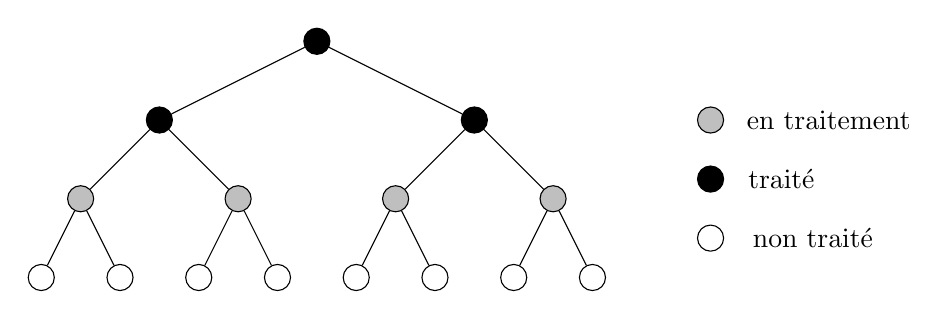
\begin{tikzpicture}
%%%%%%%%%%%%%%%%%%%%%%%%%%%%%%%%%%%%%%%%%%%%%%%%%%%%%%%%
% STYLE
\tikzstyle{processor}=[rectangle,draw]
\tikzstyle{b}=[circle,draw]
\tikzstyle{bc}=[circle,draw,fill=gray!50]
\tikzstyle{bt}=[circle,draw,fill=black]
\tikzstyle{txt}=[]

%%%%%%%%%%%%%%%%%%%%%%%%%%%%%%%%%%%%%%%%%%%%%%%%%%%%%%%%
% NODES
\node[bt] (N00) at (0,0) {};

\node[bt] (N10) at (-2,-1) {};
\node[bt] (N11) at (2,-1) {};

\node[bc] (N20) at (-3,-2) {};
\node[bc] (N21) at (3,-2) {};
\node[bc] (N22) at (-1,-2) {};
\node[bc] (N23) at (1,-2) {};

\node[b] (N30) at (-3.5,-3) {};
\node[b] (N31) at (3.5,-3) {};
\node[b] (N32) at (-1.5,-3) {};
\node[b] (N33) at (1.5,-3) {};
\node[b] (N34) at (-2.5,-3) {};
\node[b] (N35) at (2.5,-3) {};
\node[b] (N36) at (-0.5,-3) {};
\node[b] (N37) at (0.5,-3) {};

\node[bc] (L0) at (5,-1) {};
\node[bt] (L1) at (5,-1.75) {};
\node[b] (L2) at (5,-2.5) {};

\node[txt] (t5) at (6.5,-1) {en traitement};
\node[txt] (t6) at (5.9,-1.75) {traité};
\node[txt] (t7) at (6.3,-2.5) {non traité};
%%%%%%%%%%%%%%%%%%%%%%%%%%%%%%%%%%%%%%%%%%%%%%%%%%%%%%%%
% LINKS
\draw (N00) -- (N10);
\draw (N00) -- (N11);

\draw (N10) -- (N20);
\draw (N10) -- (N22);
\draw (N11) -- (N21);
\draw (N11) -- (N23);

\draw (N20) -- (N30);
\draw (N21) -- (N31);
\draw (N22) -- (N32);
\draw (N23) -- (N33);
\draw (N20) -- (N34);
\draw (N21) -- (N35);
\draw (N22) -- (N36);
\draw (N23) -- (N37);

\end{tikzpicture}
\caption*{Schématisation de \emph{blocage} des threads dans l'arbre de récursivité avec $4$ threads}
\end{figure}

Avec les $8$ processeurs du serveur, pour les $4$ premiers niveaux de l'arbre, on peut tout faire en parallèle, mais pour la suite, (n'ayant que $8$ processeurs, il ne peut y avoir réellement que $8$ thread actifs en même temps) c'est comme si il n'y avait qu'un thread (en terme de performance) pour tout le traitement de son sous-arbre, ce qui s'apparente à du séquentiel. Ainsi la durée de la descente dans l'arbre (sans compter la recherche binaire) est en $log(8) + \frac{n}{8}$.

On obtient finalement une durée totale :
\begin{equation} \label{eq-q2}
\begin{split}
T_\infty(n) & = log \, n \times (log \, 8 + \frac{n}{8})\\ 
 & = \Theta (n \times log \, n)
\end{split}
\end{equation}
 ce qui est plus grand que la durée du programme séquentiel.